This chapter provides examples that demonstrate the functionality of the \texttt{\getsoftwarename{}} application.

\section{One-story two-dimensional portal frame}

In this example, the performance of a simple 2D portal frame model is evaluated. This is an extension of the example in the EE-UQ App.\\

The model is a linear elastic single-bay single-story model of a reinforced concrete portal frame (\Cref{fig:ex_1_portal_frame}). The analysis of this model considers both gravity loading and lateral earthquake loading due to El Centro earthquake (Borrego Mountain 04/09/68 0230, El Centro ARRAY \#9, 270). The original model and ground motion used in this example were obtained from example 1b in the OpenSees website, and were modified to scale the ground motion record from gravity units (g) to the model units (in/sec2). Files for this example are included with the release of the software and are available in the \texttt{Examples/01 PortalFrame2D} folder. You can load the settings shown below using \texttt{Portal2D\_input\_file.json} file. This populates all input data automatically, except for the path to external files. These will need to be updated as shown below.\\

\begin{figure}[!htbp]
  \centering {
    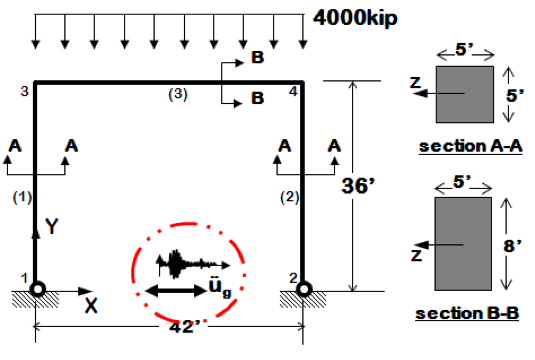
\includegraphics[width=0.8\textwidth]
    {ver_and_val/figures/portalFrame.png} }
  \caption{Two-dimensional portal frame model subjected to gravity and earthquake loading}
  \label{fig:ex_1_portal_frame}
\end{figure}

The GI and SIM setup is shown in \Cref{fig:ex_1_GI} and \Cref{fig:ex_1_SIM}. Most of the GI data are arbitrary for this example, except for the plan area that is used to estimate injuries later. Note:  the plan area is defined in square inches following the length units specified in the GI.\\

\begin{figure}[!htbp]
  \centering {
    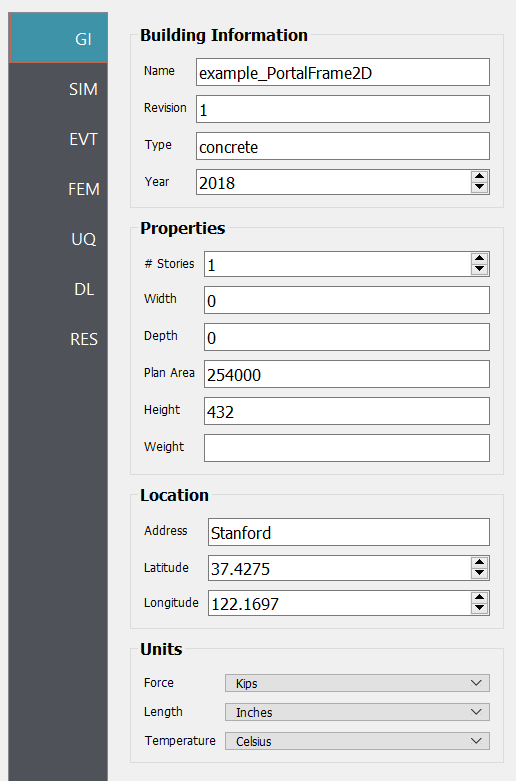
\includegraphics[width=0.4\textwidth]
    {examples/figures/ex_1_GI.png} }
  \caption{General Information about the building.}
  \label{fig:ex_1_GI}
\end{figure}

The SIM input panel requires additional input because you need to specify the location of the \texttt{Portal2D-UQ.tcl} script that describes the simulation model. The file is located in the \texttt{01 PortalFrame2D} folder. Use the \texttt{Choose} button to select the file.\\

\begin{figure}[!htbp]
  \centering {
    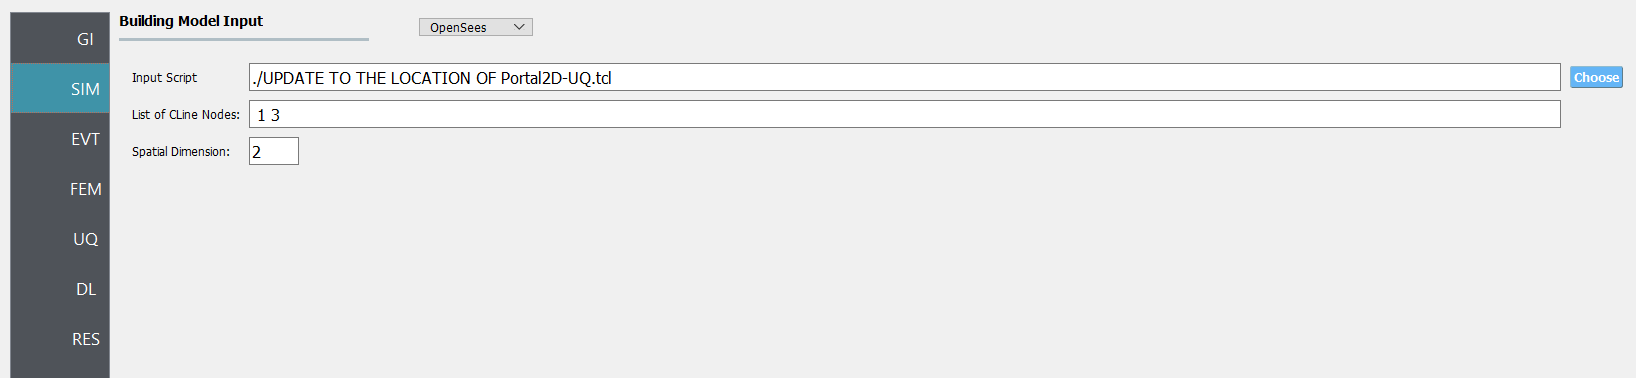
\includegraphics[width=1.0\textwidth]
    {examples/figures/ex_1_SIM.png} }
  \caption{Information about the simulation model.}
  \label{fig:ex_1_SIM}
\end{figure}

The EVT input panel in \Cref{fig:ex_1_EVT} shows that we are going to use a pre-defined \texttt{JSON} file to specify a ground motion record. You need to use the \texttt{Choose} button here to update the file location – the \texttt{BM68elc.json} file is available in the \texttt{01 PortalFrame2D} folder.\\

\begin{figure}[!htbp]
  \centering {
    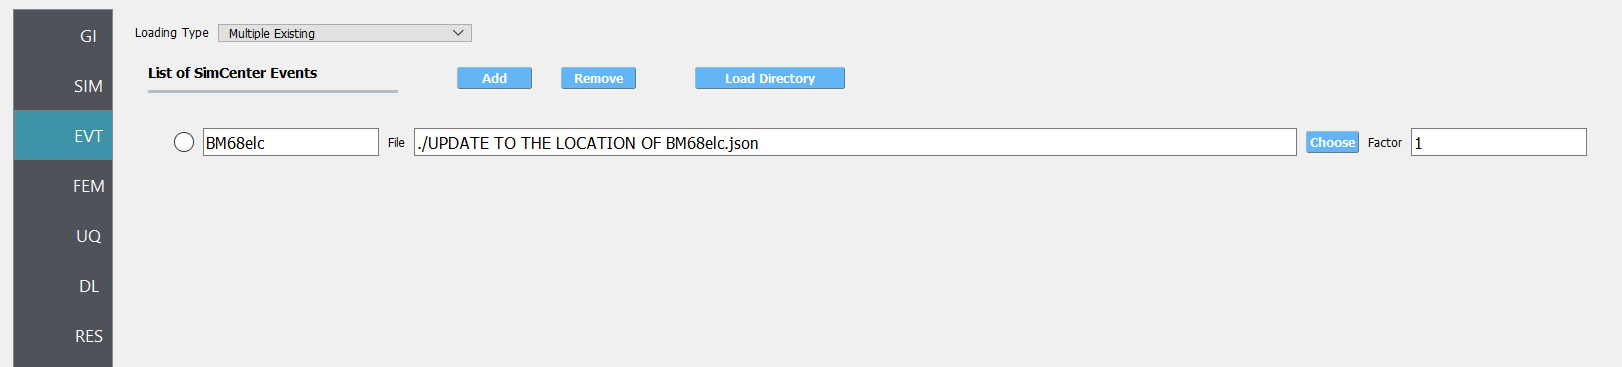
\includegraphics[width=1.0\textwidth]
    {examples/figures/ex_1_EVT.png} }
  \caption{Information about the ground motion event.}
  \label{fig:ex_1_EVT}
\end{figure}

The FEM panel contains the default settings and there is no need to change those. The UQ panel allows you to specify the number of samples (we use 10 by default) and the distribution of random variables. To introduce uncertainty in the model, the mass and the Young’s modulus are assumed to be normally distributed random variables with means and standard deviation values shown in \Cref{fig:ex_1_UQ}.\\

\begin{figure}[!htbp]
  \centering {
    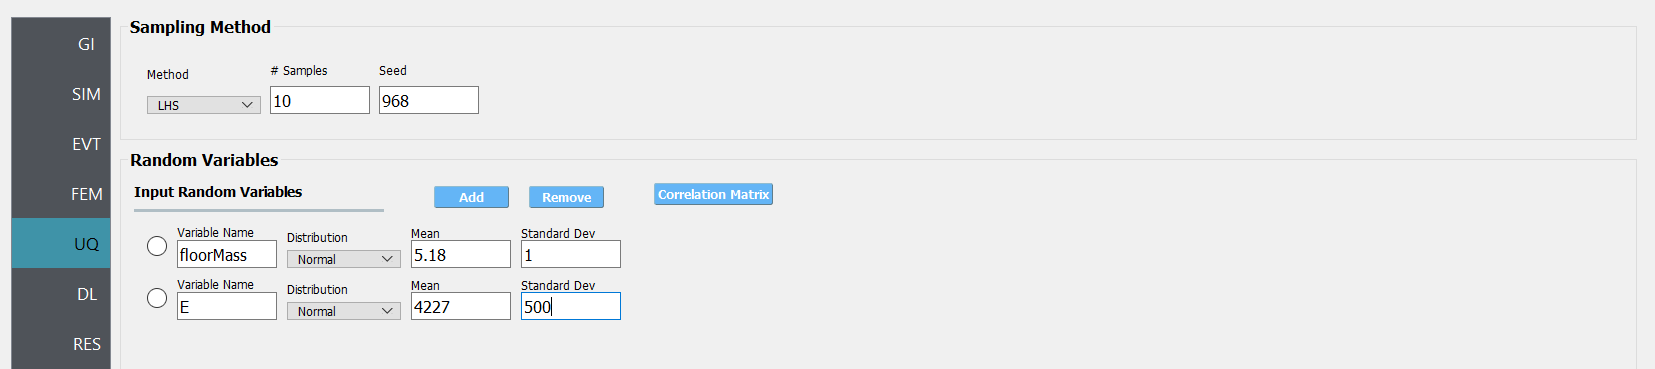
\includegraphics[width=1.0\textwidth]
    {examples/figures/ex_1_UQ.png} }
  \caption{Uncertainty quantification settings.}
  \label{fig:ex_1_UQ}
\end{figure}

A simple damage and loss model is prepared for this example (\Cref{fig:ex_1_DL_1}). We request 10,000 realizations with moderate levels of additional uncertainty. The building is assumed to be a retail area with customers inside. Hence, we specify 40 people as the peak population. The replacement cost is set to \$300,000 and the replacement time is almost a year. No dependencies are set for this example and the components are chosen from the default FEMA P58 database.\\

\begin{figure}[!htbp]
  \centering {
    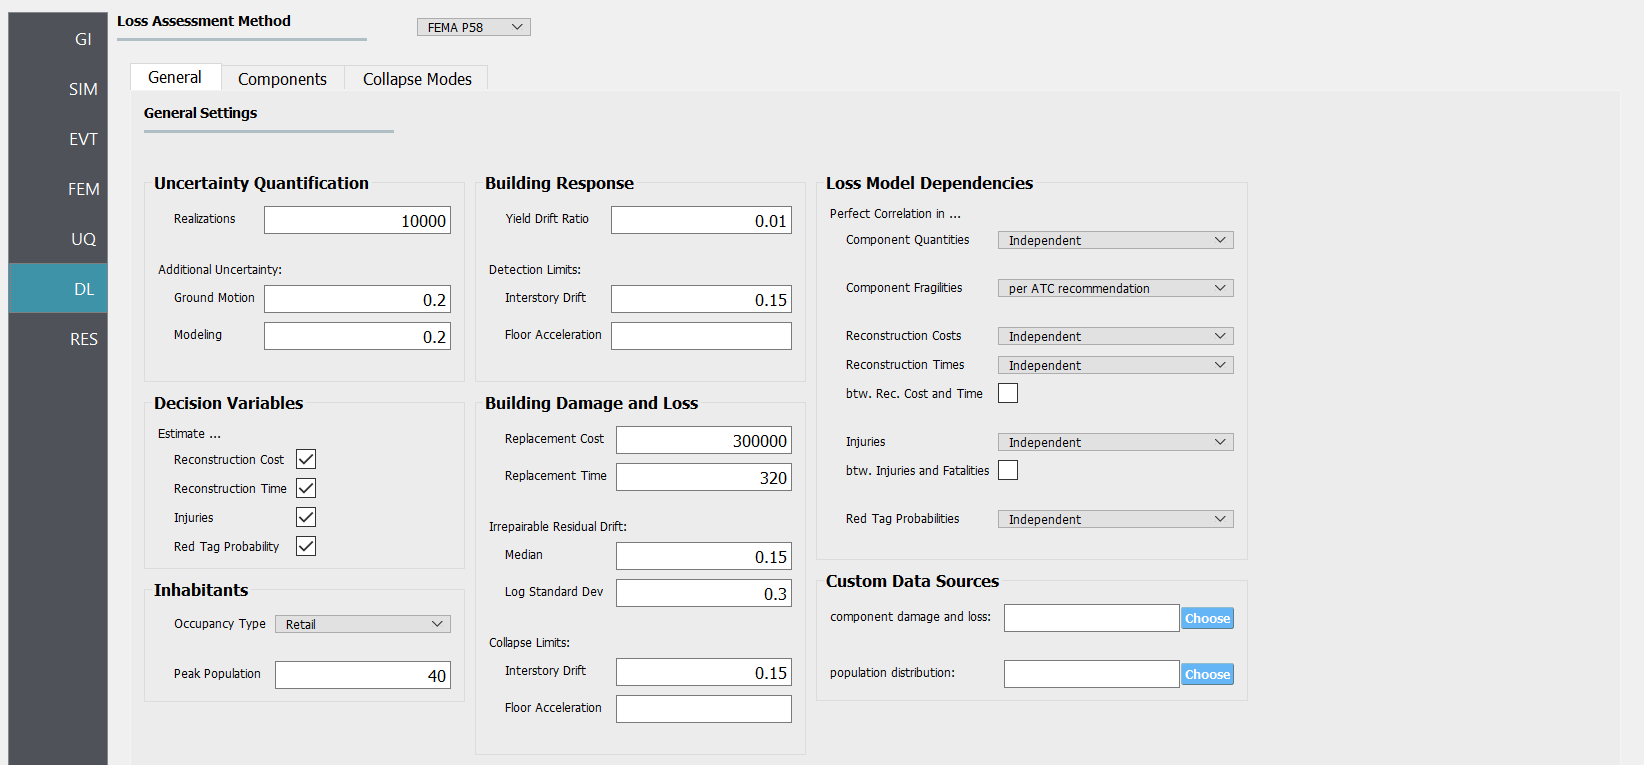
\includegraphics[width=1.0\textwidth]
    {examples/figures/ex_1_DL_1.png} }
  \caption{General settings for the Damage and Loss model.}
  \label{fig:ex_1_DL_1}
\end{figure}

The list of building components are shown in \Cref{fig:ex_1_DL_2}. NoteL the quantity fields contain only one number because the building has only one story. Multi-story buildings would need to have their component quantities specified on every floor in this panel. The units of each quantity are available in the \texttt{JSON} files in the \texttt{applications/performDL/resources/FEMA P58 first edition/DL json} folder. Future versions of the PBE App will load the information about units automatically. The data under directions not only defines the direction of each group of components, but also specifies the number of component groups in a performance group. Note that the storefront, for example, is assumed to be only on one side, hence the identical directions, but it is separated into three groups of components. The quantity corresponding to each group of components is identified by the weights. In the storefront example the weights show an uneven distribution of quantity among the three component groups.\\

\begin{figure}[!htbp]
  \centering {
    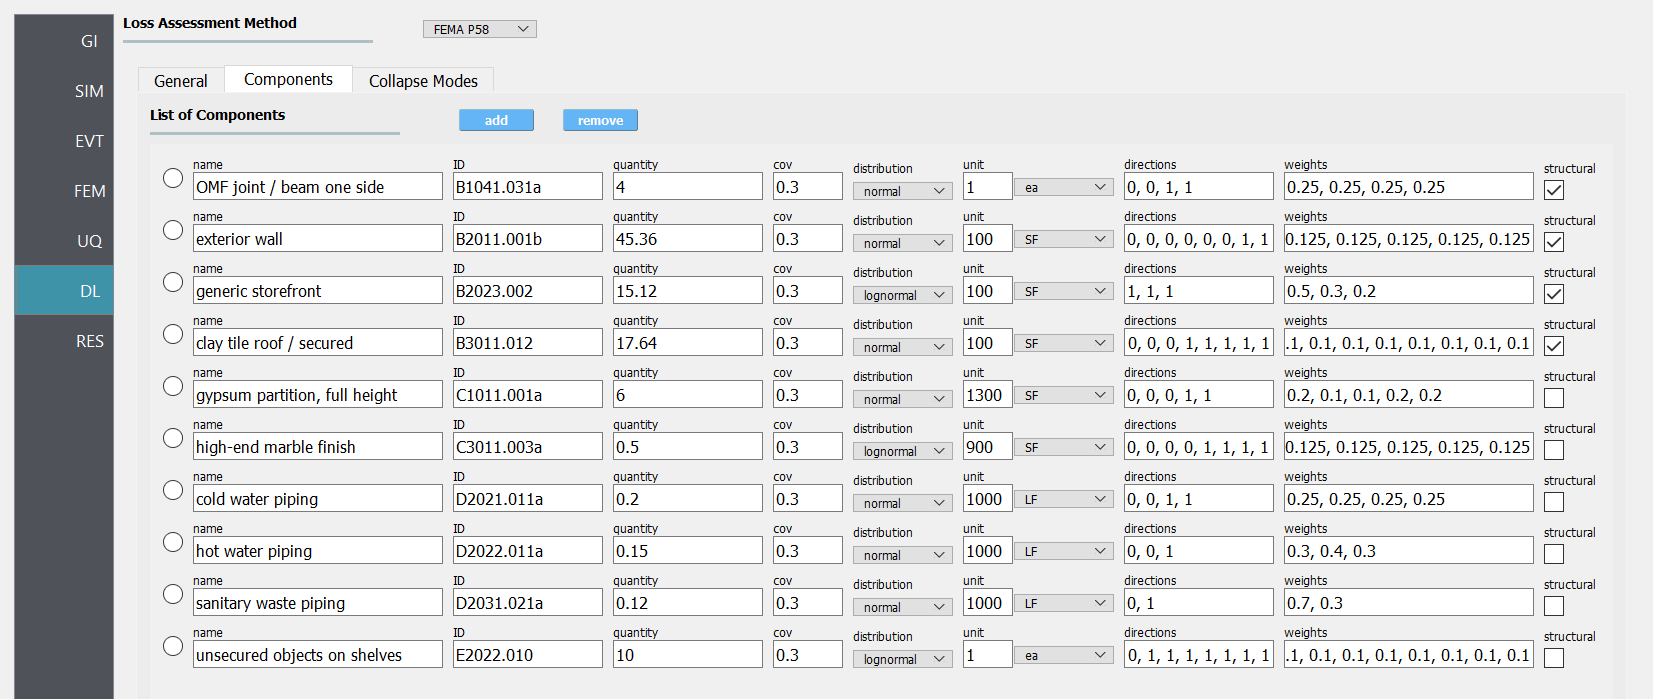
\includegraphics[width=1.0\textwidth]
    {examples/figures/ex_1_DL_2.png} }
  \caption{Component information.}
  \label{fig:ex_1_DL_2}
\end{figure}

The last tab in the DL panel identifies the collapse modes of the structure (\Cref{fig:ex_1_DL_3}). We defined two collapse modes for this example: a complete one that results mostly in fatalities and a partial one that leads to injuries in a smaller affected area and leaves most people unharmed.\\

\begin{figure}[!htbp]
  \centering {
    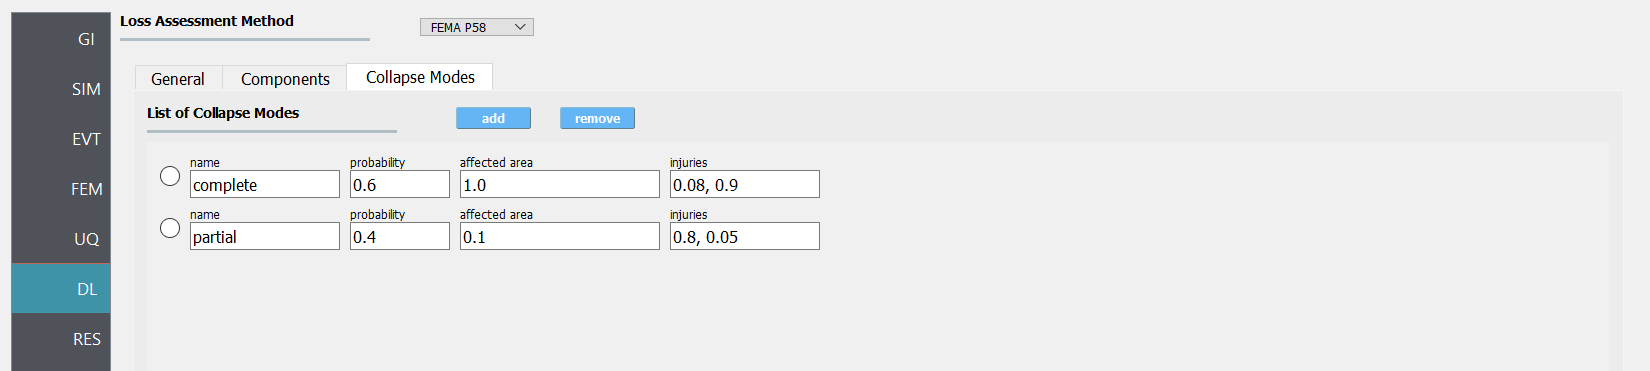
\includegraphics[width=1.0\textwidth]
    {examples/figures/ex_1_DL_3.png} }
  \caption{Collapse modes and their consequences.}
  \label{fig:ex_1_DL_3}
\end{figure}

At this point the PBE application has all the information required to create the workflow and run the performance assessment for the building. You can start running the calculation by clicking on the RUN button. This shows a dialog window requesting two pieces of information (\Cref{fig:ex_1_RUN}). The location of the working directory is arbitrary, but the application directory has to be the location of the application folder. This should be the place where you have the PBE executable file. After providing the data, click Submit to run the analysis. The runtime should not be more than 20 seconds. \\

If something goes wrong, go to the Working Dir Location and find the workflow-log file in the \texttt{tmp.SimCenter/templatedir} folder. Contact us, and send us the file.\\

\begin{figure}[!htbp]
  \centering {
    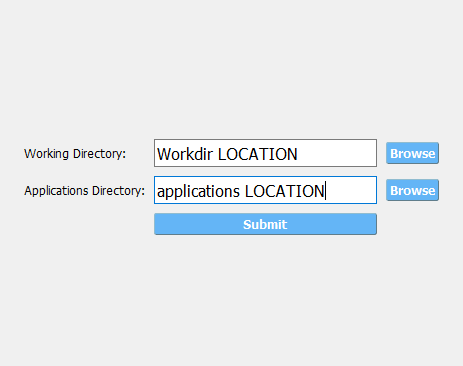
\includegraphics[width=0.5\textwidth]
    {examples/figures/ex_1_RUN.png} }
  \caption{Requested locations before running the analysis.}
  \label{fig:ex_1_RUN}
\end{figure}

If all goes well, the RES panel is automatically loaded and shows the distribution of reconstruction time among the 10,000 realizations (\Cref{fig:ex_1_RES_1}).\\

\begin{figure}[!htbp]
  \centering {
    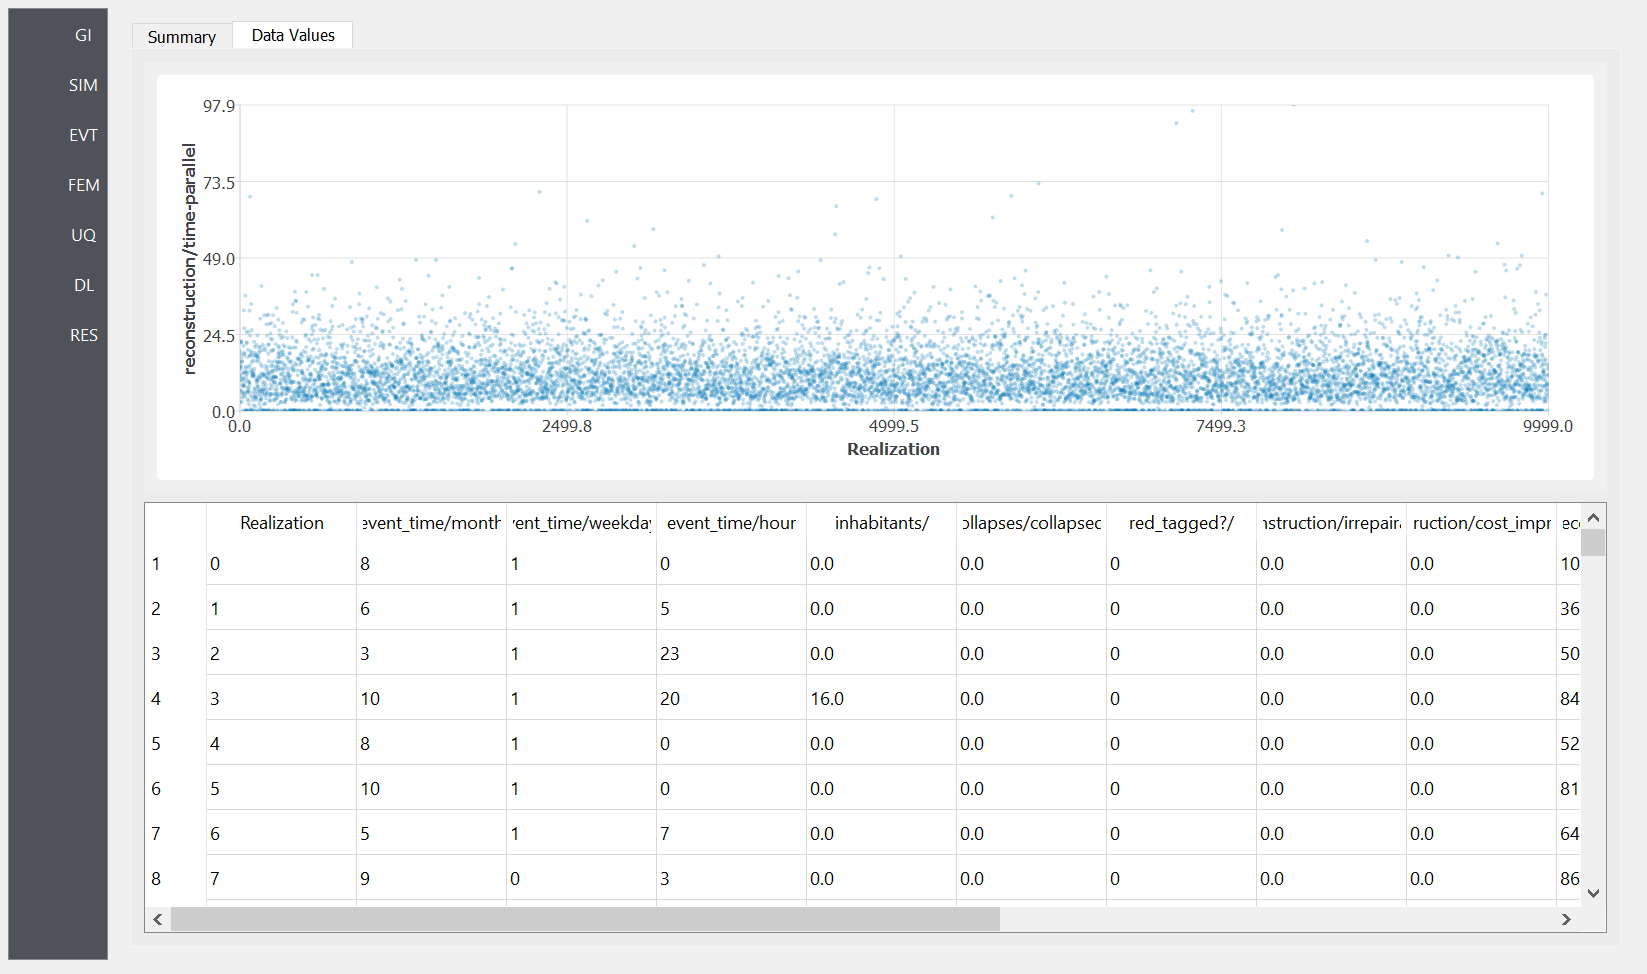
\includegraphics[width=1.0\textwidth]
    {examples/figures/ex_1_RES_1.png} }
  \caption{The RES panel after running the analysis.}
  \label{fig:ex_1_RES_1}
\end{figure}

By clicking at different columns with the left and right mouse buttons, you can visualize the relationship between decision variables, or the cumulative distribution function, or the probability density function of individual decision variables. The following figures provide a few examples.

\begin{figure}[!htbp]
  \centering {
    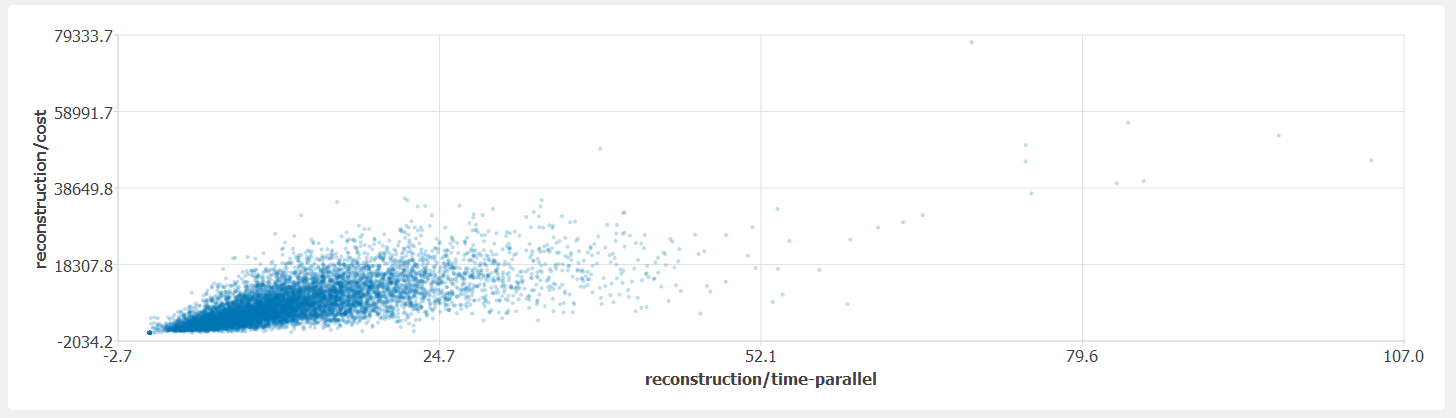
\includegraphics[width=1.0\textwidth]
    {examples/figures/ex_1_RES_2.png} }
  \caption{The joint distribution of reconstruction time (assuming parallel work) and reconstruction cost.}
  \label{fig:ex_1_RES_2}
\end{figure}

\begin{figure}[!htbp]
  \centering {
    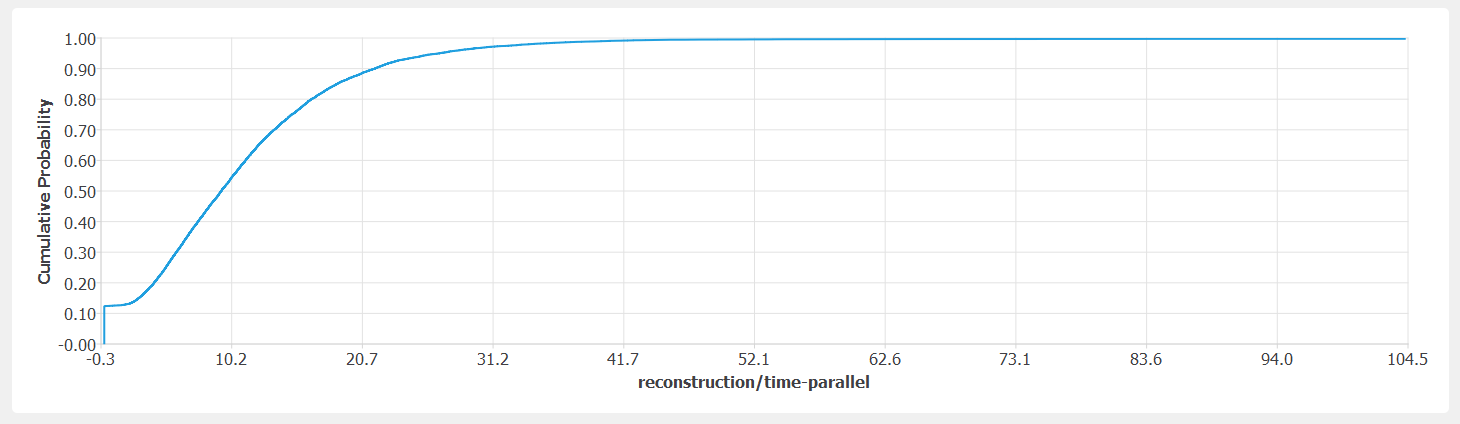
\includegraphics[width=1.0\textwidth]
    {examples/figures/ex_1_RES_3.png} }
  \caption{The cumulative distribution function of reconstruction time.}
  \label{fig:ex_1_RES_3}
\end{figure}

\begin{figure}[!htbp]
  \centering {
    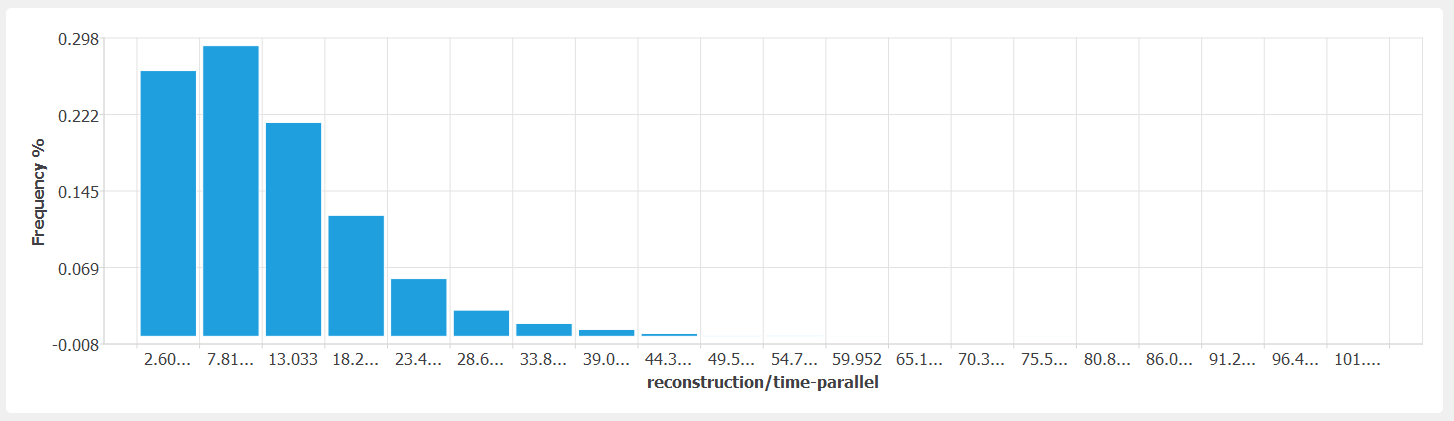
\includegraphics[width=1.0\textwidth]
    {examples/figures/ex_1_RES_4.png} }
  \caption{A histogram showing the marginal probability density function of reconstruction time.}
  \label{fig:ex_1_RES_4}
\end{figure}
